\newproblem{09a}
{
	Triangles A and B are similar.\begin{center}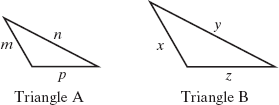
\includegraphics{fig100-09.png}\end{center} If $x=21$ in., $y=23$ in., and $m=19$ in., find the length of side $n$. Leave your answer as a fraction.
}
{
	\begin{tabular}{l r}
	$\frac{19}{21}=\frac{n}{23}$ or &  \\
	$\frac{19}{n}=\frac{21}{23}$ or& \\
	$\frac{21}{19}=\frac{23}{n}$ or &\\
	$\frac{n}{19}=\frac{23}{21}$ & 2 pts to here\\
	$n=\frac{437}{21}$ inches or $n= 20 \frac{17}{21}$ inches & 4 pts to here \\
	(3 pts for correct solution, but no units are given)
	\end{tabular}
}

\newproblem{09b}
{
	Triangles A and B are similar.\begin{center}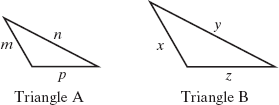
\includegraphics{fig100-09.png}\end{center} If $x=21$ in., $y=29$ in., and $m=17$ in., find the length of side $n$. Leave your answer as a fraction.
}
{
	\begin{tabular}{l r}
	$\frac{17}{21}=\frac{n}{29}$ or &  \\
	$\frac{17}{n}=\frac{21}{29}$ or& \\
	$\frac{21}{17}=\frac{29}{n}$ or &\\
	$\frac{n}{17}=\frac{29}{21}$ & 2 pts to here\\
	$n=\frac{493}{21}$ inches or $n= 23 \frac{10}{21}$ inches & 4 pts to here \\
	(3 pts for correct solution, but no units are given)
	\end{tabular}
}

\newproblem{09c}
{
	Triangles A and B are similar.\begin{center}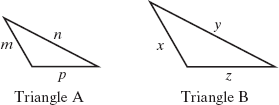
\includegraphics{fig100-09.png}\end{center} If $x=20$ in., $y=29$ in., and $m=13$ in., find the length of side $y$. Leave your answer as a fraction.
}
{
	\begin{tabular}{l r}
	$\frac{13}{20}=\frac{n}{29}$ or &  \\
	$\frac{13}{n}=\frac{20}{29}$ or& \\
	$\frac{20}{13}=\frac{29}{n}$ or &\\
	$\frac{n}{13}=\frac{20}{29}$ & 2 pts to here\\
	$n=\frac{377}{20}$ inches or $n= 18 \frac{17}{20}$ inches & 4 pts to here \\
	(3 pts for correct solution, but no units are given)
	\end{tabular}
}

\newproblem{09d}
{
	Triangles A and B are similar.\begin{center}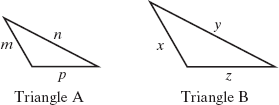
\includegraphics{fig100-09.png}\end{center} If $z=18$ in., $y=25$ in., and $n=9$ in., find the length of side $p$. Leave your answer as a fraction.
}
{
	\begin{tabular}{l r}
	$\frac{9}{25}=\frac{p}{18}$ or &  \\
	$\frac{9}{p}=\frac{25}{18}$ or& \\
	$\frac{25}{9}=\frac{18}{p}$ or &\\
	$\frac{p}{9}=\frac{18}{25}$ & 2 pts to here\\
	$p=\frac{162}{25}$ inches or $p= 6 \frac{12}{25}$ inches & 4 pts to here \\
	(3 pts for correct solution, but no units are given)
	\end{tabular}
}
